%% This is file `elsarticle-template-1-num.tex',
%%
%% Copyright 2009 Elsevier Ltd
%%
%% This file is part of the 'Elsarticle Bundle'.
%% ---------------------------------------------
%%
%% It may be distributed under the conditions of the LaTeX Project Public
%% License, either version 1.2 of this license or (at your option) any
%% later version.  The latest version of this license is in
%%    http://www.latex-project.org/lppl.txt
%% and version 1.2 or later is part of all distributions of LaTeX
%% version 1999/12/01 or later.
%%
%% Template article for Elsevier's document class `elsarticle'
%% with numbered style bibliographic references
%%
%% $Id: elsarticle-template-1-num.tex 149 2009-10-08 05:01:15Z rishi $
%% $URL: http://lenova.river-valley.com/svn/elsbst/trunk/elsarticle-template-1-num.tex $
%%
\documentclass[preprint,12pt]{elsarticle}

%% Use the option review to obtain double line spacing
%% \documentclass[preprint,review,12pt]{elsarticle}

%% Use the options 1p,twocolumn; 3p; 3p,twocolumn; 5p; or 5p,twocolumn
%% for a journal layout:
%% \documentclass[final,1p,times]{elsarticle}
%% \documentclass[final,1p,times,twocolumn]{elsarticle}
%% \documentclass[final,3p,times]{elsarticle}
%% \documentclass[final,3p,times,twocolumn]{elsarticle}
%% \documentclass[final,5p,times]{elsarticle}
%% \documentclass[final,5p,times,twocolumn]{elsarticle}

%% The graphicx package provides the include graphics command.
\usepackage{graphicx}
%% The amssymb package provides various useful mathematical symbols
\usepackage{amssymb}
%% The amsthm package provides extended theorem environments
%% \usepackage{amsthm}

%% The lineno packages adds line numbers. Start line numbering with
%% \begin{linenumbers}, end it with \end{linenumbers}. Or switch it on
%% for the whole article with \linenumbers after \end{frontmatter}.
\usepackage{lineno}

%% package to disable splite word at the end of a line
%% use \sloppy{} at the begining of each section to re-arrange the space between each word in each line, other with Latex has a default space between them
\usepackage[none]{hyphenat}


%% nomenclature
\usepackage{nomencl} 
\makenomenclature

%% subgroup in nomenclature
\usepackage{etoolbox}


%% natbib.sty is loaded by default. However, natbib options can be
%% provided with \biboptions{...} command. Following options are
%% valid:

%%   round  -  round parentheses are used (default)
%%   square -  square brackets are used   [option]
%%   curly  -  curly braces are used      {option}
%%   angle  -  angle brackets are used    <option>
%%   semicolon  -  multiple citations separated by semi-colon
%%   colon  - same as semicolon, an earlier confusion
%%   comma  -  separated by comma
%%   numbers-  selects numerical citations
%%   super  -  numerical citations as superscripts
%%   sort   -  sorts multiple citations according to order in ref. list
%%   sort&compress   -  like sort, but also compresses numerical citations
%%   compress - compresses without sorting
%%
%% \biboptions{comma,round}

% \biboptions{}



\journal{Chemical Engineering Journal}

\begin{document}
% \mbox{}
\begin{frontmatter}

%% Title, authors and addresses

\title{Flow Pattern and Boosting Pressure Prediction of Electrical Submersible Pump (ESP) in Gas-Liquid Flow}

%% use the tnoteref command within \title for footnotes;
%% use the tnotetext command for the associated footnote;
%% use the fnref command within \author or \address for footnotes;
%% use the fntext command for the associated footnote;
%% use the corref command within \author for corresponding author footnotes;
%% use the cortext command for the associated footnote;
%% use the ead command for the email address,
%% and the form \ead[url] for the home page:
%%
%% \title{Title\tnoteref{label1}}
%% \tnotetext[label1]{}
%% \author{Name\corref{cor1}\fnref{label2}}
%% \ead{email address}
%% \ead[url]{home page}
%% \fntext[label2]{}
%% \cortext[cor1]{}
%% \address{Address\fnref{label3}}
%% \fntext[label3]{}


%% use optional labels to link authors explicitly to addresses:
%% \author[label1,label2]{<author name>}
%% \address[label1]{<address>}
%% \address[label2]{<address>}

\author{Haiwen Zhu\textsuperscript{a}, Jianjun Zhu\textsuperscript{b*}, and Hong-Quan Zhang\textsuperscript{a}}
%% 页脚?? corresponding author
\address{a McDougall School of Petroleum Engineering, The University of Tulsa, 800 S Tucker Dr, Tulsa, OK, 74104}
\address{b College of Mechanical and Transportation Engineering, China University of Petroleum-Beijing, Beijing, 102249, China}
\begin{abstract}
    %% re-arrange the space between each word in each line
    \sloppy{}
%% Text of abstract
The performance of widely used Electrical Submersible Pump (ESP) is significantly affected by gas entrainment, which is an encountered phenomenon in the petroleum industry. The boosting pressure of an ESP gradually degrades with the increase of inlet gas void fraction (GVF). The flow becomes unstable and a breakdown occurs when the flow pattern switches from bubble flow to intermittent flow. Therefore, an accurate ESP model is necessary to help design and operate the ESP system under gassy flow conditions. The gas-liquid two-phase tests of different ESPs were extensively carried out at the Tulsa University Artificial Lift Projects (TUALP) to investigate the complex flow behaviors. Then, a mechanistic model was proposed for the gas-liquid flow inside a rotating ESP, which captures the gas-liquid two-phase flow characteristics, including in-situ gas void fraction, flow pattern transition, bubble size, boosting pressure, etc. 

In the new model, the pump head is calculated by subtracting recirculation head loss, turning head loss, friction head loss, and friction head loss from Euler head. The recirculation head loss is estimated by a new theory, the best-match flowrate \textit{$Q_{BM}$}. It is generated by the mismatch of the velocity of real flowrates and \textit{$Q_{BM}$}. The drag force coefficient correlations are selected and improved based on flow patterns and bubble sizes. Then, the mixture density and in-situ gas void fraction are calculated according to the force balance on gas bubbles. The proposed model is validated by experimental data of a radial-type ESP (TE2700) and two mixed-type ESPs (GC6100 and MTESP) in the TUALP database. The predicted ESP boosting pressures and flow patterns agree well with the corresponding experimental measurements.

\end{abstract}
\begin{keyword}
Artificial Lift \sep Electrical Submersible Pump (ESP) \sep Gas-Liquid Flow \sep Experiments \sep Mechanistic Modeling
%% keywords here, in the form: keyword \sep keyword

%% MSC codes here, in the form: \MSC code \sep code
%% or \MSC[2008] code \sep code (2000 is the default)

\end{keyword}

\end{frontmatter}

%%
%% Start line numbering here if you want
%%
\linenumbers

%% main text
\section{Introduction}
\sloppy{}
\label{S:Introduction}

The electrical submersible pumps (ESPs), with more than 200,000 installations, are widely used in the petroleum industry, especially in the offshore fields with high production rates \cite{zhu2017phd}. However, complex flow conditions, including high viscosity oil, gas, and sand, jeopardize ESP performance and reduce its lifespan. The internal multiphase flow structure is difficult to be characterized due to its complex geometry, resulting in obstacles in ESP modeling. The first experiment of gas-liquid flow in a centrifugal pump was conducted by Murakami and Minemura \cite{murakami1974effects1,murakami1974effects2}, which is a visualization test with a semi-opened transparent impeller (rotor). The ESP’s hydraulic head degrades with the increase of gas entrainment, especially when gas pockets are formed. The effect of pump hydraulic parameters on its boosting pressure, including pump types \cite{cirilo1998air}, stage number \cite{pessoa2001experimental}, rotational speed \cite{zapata2003rotational}, inlet pressure \cite{salehi2012esp}, surfactant concentration \cite{zhu2018surfactant}, seal clearance \cite{zhu2019experiments}, grooves on volute \cite{shen2020study} were studied separately. At TULAP, two-phase performance experiments were extensively carried out for different ESPs, including GN7000 \cite{romero1999evaluation}, GN4000 \cite{cirilo1998air,romero1999evaluation}, GC6100 \cite{pessoa2001experimental,beltur2003analysis,duran2003pressure,zapata2003rotational,gamboa2009prediction}, DN1750 \cite{banjar2013experimental}, TE2700 \cite{salehi2012esp,zhu2017phd}, and MTESP \cite{zhu2020experimental}. Specifically, gas-liquid visualization experiments were carried out for GC6100 \cite{barrios2007visualization,gamboa2009prediction,trevisan2009modeling}.

With the understanding of gas-liquid two-phase flow characteristics inside ESPs from experimental studies, the theoretical work on calculating the ESP boosting pressure under both single-phase and gassy conditions has been conducted by researchers. Based on the ideal assumptions (incompressible, frictionless, infinite blades/vanes, static flow), Euler head has been incorporated in most existing models to estimate the boosting pressure of a centrifugal pump. The velocity triangles in an ESP impeller is shown in Figure \ref{fig:velocityTriangle}, in which the global absolute velocity $C$ is composed by impeller relative velocity $W$ and peripheral velocity $U$. Figure \ref{fig:velocityTriangle} (b) and (c) show the triangle relationship between $C$, $W$, and $U$ at the impeller inlet and outlet, where the subscript 1 and 2 represent inlet and outlet. $C’_2$ is the ideal absolute velocity assuming an infinite number of impeller blades. 

\begin{figure}[h]
    % h, here
    % t, top
    % b, bottom
    % p, page of float
    % ht, here and top
\label{fig:velocityTriangle}
\centering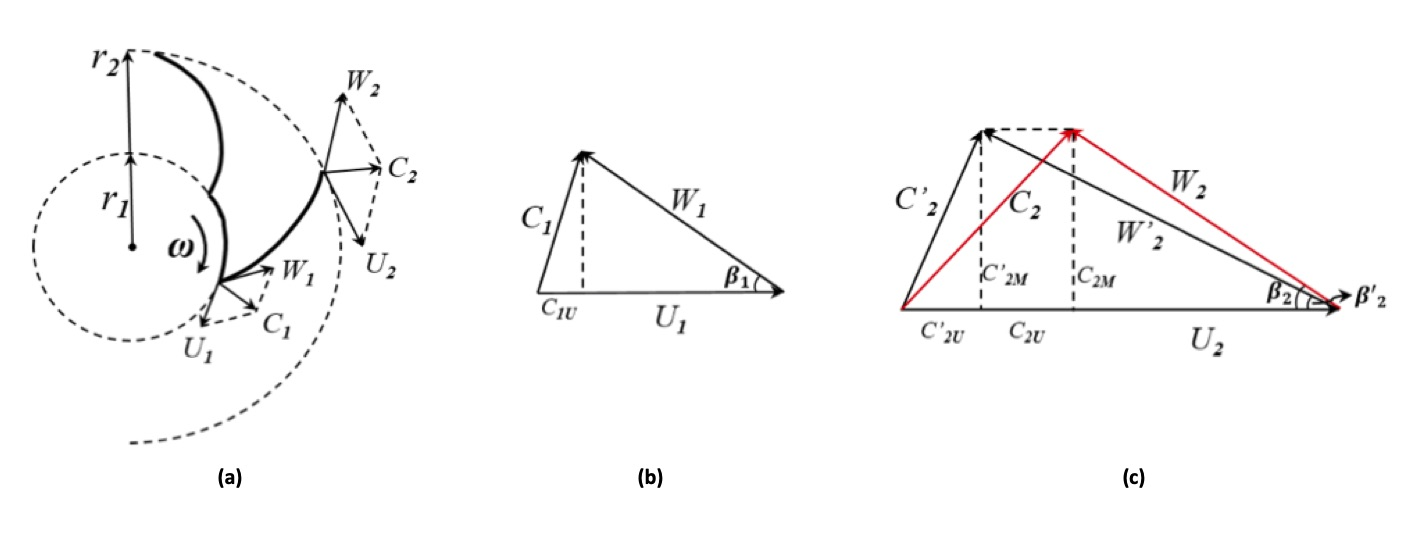
\includegraphics[width=1\linewidth]{velocity triangle.jpg}
\caption{Velocity triangles in an ESP impeller, (a) impeller flow channel, (b) inlet velocity triangle, (c) outlet velocity triangle.}
\end{figure}

Stepanoff (1958) introduced the Euler head ($H_E$) that developed based on the ideal angular momentum conservation equations in centrifugal pumps as:

\begin{equation}
    \label{eq:HeOriginal}
    H_E = \frac{\vec C_2\cdot\vec U_2-\vec C_1\cdot\vec U_1}{g}=\frac{C_2U_{2U}-C_1U_{1U}}{g}
\end{equation}
where the subscript $U$ represents the peripheral direction. According to the velocity triangles in Figure \ref{fig:velocityTriangle}, the Euler head can be re-writen as:
\begin{equation}
    \label{eq:HeModified}
    H_E = \frac{U_2^2-U_2^2}{2g}-\frac{W_2^2-W_2^2}{2g}-\frac{C_2^2-C_2^2}{2g}
\end{equation}
and
\begin{equation}
    \label{eq:HeModified2}
    H_E = \frac{\Omega^2(r_2^2-r_1^2)}{g}-\frac{Q\Omega}{2\pi gh}(\frac{1}{\tan{\beta_2}}-\frac{1}{\tan{\beta_1}})
\end{equation}
where $r$ is the radius of the impeller, $h$ is the channel height, $\beta$ is the blade angle from the tangential direction. If $\beta_1$ is close to ${90^{\circ}}$ or the fluids enter the impeller without pre-rotation, Equation \ref{eq:HeModified2} can be written as
\begin{equation}
    \label{eq:Hefinal}
    H_E=\frac{\Omega^2r_2^2}{g}-\frac{Q\Omega}{2\pi gh \tan{\beta_2}}
\end{equation}

Then, the relationship between the ideal Euler head and outlet blade angle $\beta_2$ is shown in Figure 2 (a). The real pump head is calculated by subtracting the head losses in Figure \ref{fig:velocityTriangle} (b) from the Euler head in Equation \ref{eq:Hefinal} as: 
\begin{equation}
    \label{eq:headall}
    H=H_E-H_{friction}-H_{shock}-H_{leakage}-H_{recirculation}-H_{diffuser}-H_{disk}
\end{equation}

\begin{figure}[ht]
    \label{fig:headLossType}
    \centering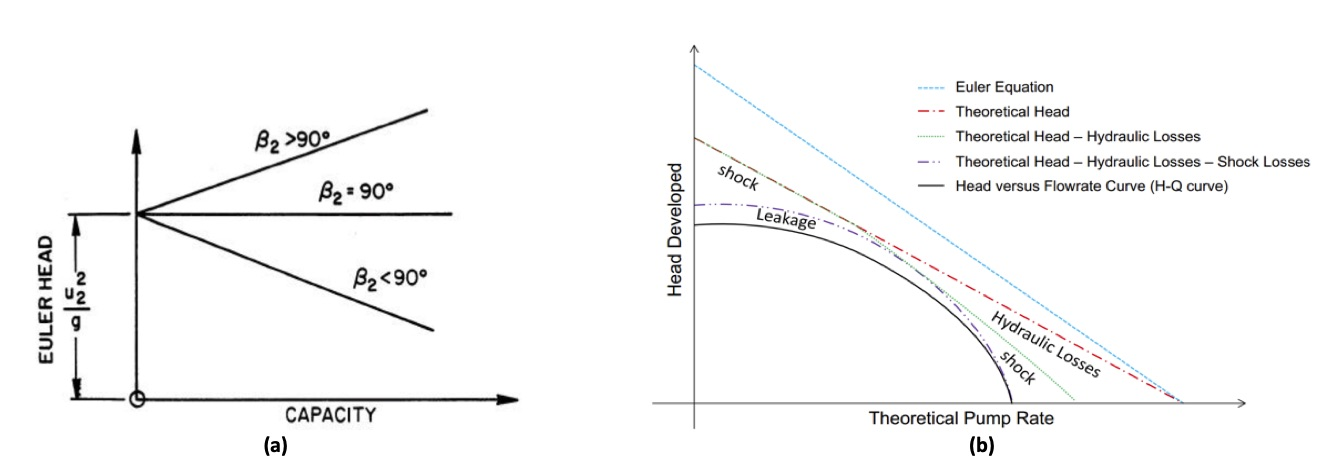
\includegraphics[width=1\linewidth]{head loss type.jpg}
    \caption{Schematic of head curves, (a) Euler head with different outlet blade angles, (b) actual head after deducting losses (Vieira et al., 2015).}
\end{figure}

The remaining difficulty is to determine different types of head loss and gas effect to mixture density in an impeller. For two-phase modeling of gas-liquid performance inside a rotating centrifugal pump, several one-dimensional (1D) two-fluid models have been proposed in the literature. In 1980, a 1D control volume method was proposed by Zakem to analyze the gas-liquid interaction effect in straight channel impellers. Similarly, Furuya \cite{furuya1985analytical} established an analytical model by considering pump geometry, GVF, slippage, and flow patterns. However, the fluid compressibility and condensation effect were neglected, which results in an average error of $\pm{30\%}$ for GVF $< 20\%$ and $\pm50\%$ for GVF $> 30\%$. Then a comprehensive investigation of ESP two-phase flow, including air-water and diesel-CO\textsubscript{2}, was carried out by Sachdeva et al. \cite{sachdeva1988two,sachdeva1994performance}, based on which a dynamic five-equation, 1D, two-fluid model was developed and validated. Besides, Minemura et al. \cite{minemura1998prediction} developed a two-phase model for centrifugal pumps based on energy changes from rotating impeller and stationary volute, which considers fluid viscosity effect and gas compressibility. Although pump geometry and momentum balance equations are included in Minemura et al. \cite{minemura1998prediction} and Sachdeva et al. \cite{sachdeva1994performance} models, they are restricted to narrow experimental flow conditions and pump types. Based on their studies, Sun \cite{sun2003,sun2005modeling} and improved correlations for head losses and drag coefficient, and developed a new two-phase model based on mixed-type GC6100 testing results at TUALP by solving a set of 1D conservation equations. However, the model cannot predict the boosting pressure of radial-type TE2700 under two-phase flow conditions with acceptable accuracy. 

Although experimental and theoretical studies on ESP under gassy flow are introduced, most of them are only validated by their pump and testing conditions. The flow pattern transition, gas-liquid slippage, gas bubble size effect on in-situ gas void fraction and mixture density in ESPs are not well understood. Mechanistic modeling of ESP two-phase performance is still preliminary in the literature. Experimental investigations are insufficient on ESP two-phase flow behaviors including flow patterns and transition boundaries. The development and validations are also critical for the accuracy of model predictions. In this paper, a mechanistic model is proposed to predict the flow patterns and boosting pressure under gas-liquid flow inside a rotating ESP. The model, validated by the three pump curves in the TUALP database, including 5-inch mixed-type GC6100 \cite{gamboa2009prediction}, 5-inch radial-type TE2700 \cite{zhu2017phd}, and 4-inch mixed-type MTESP \cite{zhu2020experimental}, can capture the multiphase flow characteristics, such as flow pattern transition, in-situ gas void fraction $\aleph_G$, bubble sizes, etc. The predicted ESP boosting pressure of three ESPs shows good agreement with the experimental data. 



\section{Model Development}
\label{S:Model Development}
This section discusses the mechanistic model for predicting ESP performance, including single-phase liquid and gas-liquid two-phase modeling, as well as the closure relationships for estimating the representative bubble size, the in-situ gas void fraction $\alpha_G$, and drag coefficient, etc. Meanwhile, the comparisons of mechanistic model predictions with corresponding experimental data are also presented.

\subsection{Single-phase Liquid Performance}
Takacs \cite{takacs2017electrical} listed three head loss types in centrifugal pumps, namely hydraulic losses, shock losses, and leakage losses. The actual pump head is the result after subtracting all the head losses from Euler head. The hydraulic losses caused by fluid friction and diffusion losses inside impeller channels increase steadily with the liquid flow rate. The shock losses are negligible at the best efficient point (BEP) but increase at lower or higher liquid rates, which is due to sudden changes in flow direction at the inlet and outlet of the impeller. The leakage losses always exist as long as the liquids flow through the clearances between the rotating and stationary parts of the pump stage, including the impeller eye, balancing holes. However, the leakage losses diminish with the increased liquid flow rates due to lower backpressures.

In this study, the mechanistic model of ESP boosting pressure starts from Euler equation and introduces a conceptual best match flow rate ($Q_{BM}$), at which the flow direction at the impeller outlet matches the designed flow direction. The recirculation head loss is calculated by the mismatch of the velocity triangles compared to the $Q_{BM}$.

\subsubsection{Liquid Flow Rate $Q_l < Q_{BM}$}
Based on the velocity triangles in Figure 1, three terms at the right-hand side (RHS) of Equation \ref{eq:HeModified} are the hydraulic heads as a consequence of centrifugal force, velocity change through the impeller as well as dynamic effect, respectively. For each velocity component, its expression is discussed below. The tangential velocity at the impeller inlet is given by
\begin{equation}
    \label{eq:U1}
    U_1=R_1\Omega
\end{equation}
where $R_1$ is the radius of the impeller inlet, and $\Omega$ is the angular velocity of the impeller. Similarly, the tangential velocity at the impeller outlet is expressed as
\subsubsection{Liquid Flow Rate $Q_l > Q_{BM}$}

\subsubsection{Friction Loss}
\subsubsection{Leakage Loss}
\subsection{Gas-Liquid Performance}
\subsubsection{Closure Relationships}

\section{Results and Discussions}
\begin{table}[h]
    \centering
    \begin{tabular}{l l l}
    \hline
    \textbf{Treatments} & \textbf{Response 1} & \textbf{Response 2}\\
    \hline
    Treatment 1 & 0.0003262 & 0.562 \\
    Treatment 2 & 0.0015681 & 0.910 \\
    Treatment 3 & 0.0009271 & 0.296 \\
    \hline
    \end{tabular}
    \caption{Table caption}
    \end{table}
\subsection{Single-phase Flow Results}

\subsection{Gas/Liquid Two-phase Flow Results}

\subsubsection{Mapping Test Results}
\subsubsection{Surging Test Results}

\section{Conclusions}

% \section{Nomenclature}

%% This will add the subgroups
%----------------------------------------------
\renewcommand\nomgroup[1]{
  \item[\bfseries
  \ifstrequal{#1}{A}{General}{
  \ifstrequal{#1}{B}{Greek Symbols}{
  \ifstrequal{#1}{C}{Subscripts}{}}}
]}
%----------------------------------------------

%% This will add the units
%----------------------------------------------
\newcommand{\nomunit}[1]{
    \renewcommand{\nomentryend}{\hspace*{\fill}#1}}
    %----------------------------------------------
%----------------------------------------------
\mbox{}

\nomenclature[A, 02]{$c$}{Speed of light in a vacuum inertial system 
  \nomunit{$299,792,458\, m/s$}}
\nomenclature[A, 03]{$h$}{Plank Constant
  \nomunit{$6.62607 \times 10^{-34}\, Js$}}
\nomenclature[A, 01]{$g$}{Gravitational Constant 
  \nomunit{$6.67384 \times 10^{-11}\, N \cdot m^2/kg^2$}}
\nomenclature[B, 03]{$\mathbb{R}$}{Real Numbers}
\nomenclature[B, 02]{$\mathbb{C}$}{Complex Numbers
    \nomunit{$6.67384 \times 10^{-11}\, N \cdot m^2/kg^2$}}
\nomenclature[B, 01]{$\mathbb{H}$}{Quaternions}
\nomenclature[C]{$V$}{Constant Volume\nomunit{m}}
\nomenclature[C]{$\rho$}{Friction Index\nomunit{m}}

\printnomenclature

\section*{Acknowledgements}
The authors appreciate Tulsa University Artificial Lift Projects (TUALP) members’ financial and technical support, as well as providing pumps for experiments. 

%% References
%%
%% Following citation commands can be used in the body text:
%% Usage of  \cite is as follows:
%%    \cite{key}          ==>>  [#]
%%    \cite[chap. 2]{key} ==>>  [#, chap. 2]
%%    \citet{key}         ==>>  Author [#]

%% References with bibTeX database:

% \bibliographystyle{model1-num-names}

%% New version of the num-names style
\bibliographystyle{elsarticle-num-names}
\bibliography{bibliography.bib}

%% Authors are advised to submit their bibtex database files. They are
%% requested to list a bibtex style file in the manuscript if they do
%% not want to use model1-num-names.bst.

%% References without bibTeX database:

% \begin{thebibliography}{00}

%% \bibitem must have the following form:
%%   \bibitem{key}...
%%

% \bibitem{}

% \end{thebibliography}


% \begin{itemize}
% \item Bullet point one
% \item Bullet point two
% \end{itemize}

% \begin{enumerate}
% \item Numbered list item one
% \item Numbered list item two
% \end{enumerate}

%% The Appendices part is started with the command \appendix;
%% appendix sections are then done as normal sections
% \appendix

% \section{example}
% \label{A:1}

% appendix example



\end{document}

%%
%% End of file `elsarticle-template-1-num.tex'.